\centerline{\bf \Huge МатДрака}

\problem{\textbf{1}} У НеНачальника было 2025 пустых копилок. В некоторые из них он положил по 2025 пустых копилок и повторил эту операцию еще несколько раз. В итоге стало 2607 непустых копилок.
Сколько всего стало копилок у НеНачальника?

\problem{\textbf{2}} В тёмной комнате на полке в беспорядке лежат четыре пары носков двух разных размеров и двух разных цветов. Какое наименьшее число носков необходимо, не выходя из комнаты, переложить с полки в чемодан, чтобы в нем оказались две пары различного размера и цвета?

\problem{\textbf{3}} $50\cdot(\dfrac{(1,238+2,762) \cdot 0,1}{(36,487-34,237): 2,8125}+\dfrac{(4,36-1,16) \cdot 0,3125}{0,2 \cdot(47,8-45,55): 0,225})\cdot$ 

$\cdot(39,86-\dfrac{8 \dfrac{4}{5}}{6,934+38 \dfrac{13}{40}: 2 \dfrac{1}{2} \cdot 0,2}-17)$ = ?

\problem{\textbf{4}} У Начальника и НеНачальника есть несколько шоколадок, каждая весом не более 100 граммов. Как бы они ни поделили эти шоколадки, у одного из них суммарный вес шоколадок не будет превосходить 100 граммов. Какой наибольший суммарный вес могут иметь все шоколадки?

\problem{\textbf{5}} По окружности выписано 10 чисел, сумма которых равна 100. Известно, что сумма каждых трёх чисел, стоящих рядом, не меньше 29.
Укажите такое наименьшее число А, что в любом таком наборе чисел каждое из чисел не превосходит А.

\problem{\textbf{6}} Сколько существует пар натуральных чисел $x > y$ таких, что их
произведение на 19999 больше их суммы?


\problem{\textbf{7}} Трое играют в настольный теннис, причем игрок, проигравший партию, уступает место игроку, не участвовавшему в ней. В итоге оказалось, что первый игрок сыграл 10 партий, второй – 21. Сколько партий сыграл третий игрок?

\problem{\textbf{8}} В сериале "Тайна Санта-Барбары" участвует 20 героев. Каждую серию происходит одно из событий: некоторый герой узнаёт Тайну, некоторый герой узнаёт, что кто-то знает Тайну, некоторый герой узнаёт, что кто-то не знает Тайну. Какое наибольшее число серий может продолжаться сериал?

\newpage

\hspace{3mm}

\problem{\textbf{9}} Найдите количество четырёхзначных чисел, у которых третья цифра
меньше четвёртой на 2.


\problem{\textbf{10}} Сколькими способами можно
разместить числа 1, 2, 3, 4, 5, 6, 7, 8 и 9 в девяти клетках фигуры, изображённой на рисунке, так, чтобы сумма чисел в каждом столбце, начиная
со второго, была на 1 больше, чем в предыдущем?

\problem{\textbf{11}} Каких целых чисел от 1 до 60 000 (включительно) больше и на сколько: содержащих в своей записи только чётные цифры или содержащих в своей записи только
нечётные цифры?

\problem{\textbf{12}} Сколькими различными способами шахматный ферзь может пройти с поля d1 на поле h8, если ему разрешается ходить только вправо, вверх или по диагонали
вправо вверх на любое число клеток?

\problem{\textbf{13}} Сколько натуральных чисел, делящихся на 4 и
меньших 1000, не содержат в десятичной записи ни одной из цифр 3, 4, 5, 7 и 9?

\problem{\textbf{14}} Туристическая фирма провела акцию: «Купи путёвку в Египет,
приведи четырёх друзей, которые также купят путёвку, и получи стоимость путёвки обратно».
За время действия акции 13 покупателей пришли сами, остальных привели друзья. Некоторые
из них привели ровно по 4 новых клиента, а остальные 100 не привели никого. Сколько туристов
отправились в Страну Пирамид бесплатно?

\problem{\textbf{15}} В первенстве по футболу участвует 20 команд, которые играют по разу друг с другом. Какое наименьшее число игр должно быть сыграно, чтобы среди любых трёх команд нашлись две, уже сыгравшие между собой?

\problem{\textbf{16}}
$AB=CE$, $AD=CD$, $\angle ABC = 61^{\circ}$, $\angle DCE = 17^{\circ}$. Найдите угол $\angle BAD.$

\begin{center}
    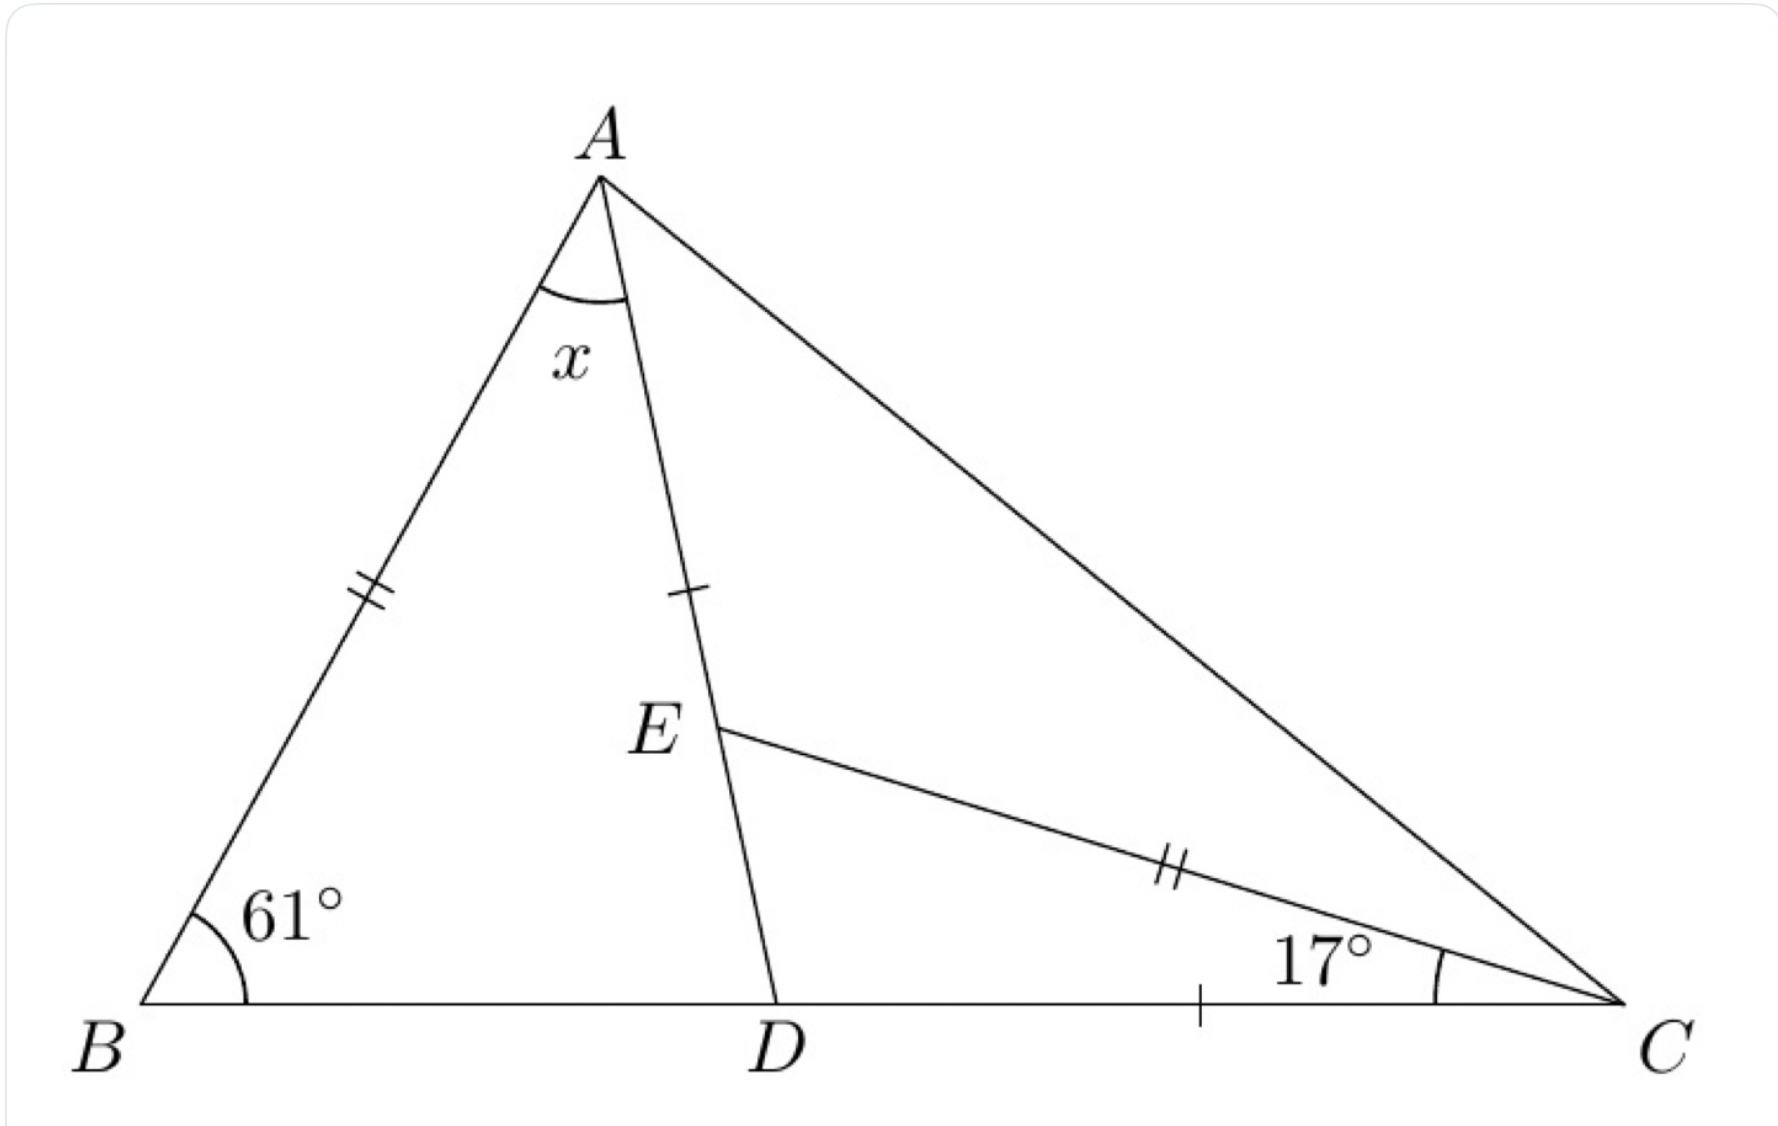
\includegraphics[width=0.45\textwidth]{Сборы/Сборы Элиста 2025/РВ/8/Матдрака I/image.png}
\end{center}